\section{Causal interventions}
\label{sec:interventions}

Everything so far has been observation. We recorded activations and found structure in them. Structure in
activations shows what \emph{could} be used by the model. To learn what \emph{is} used, we have to change an
activation and see whether the output changes. A neural network is an unusually good object for this kind of
experiment. We can set any internal quantity to any value, rerun the rest of the computation exactly, and
repeat as often as we like.

\subsection{Interventions and ablations}

\begin{definition}[Intervention]\label{def:intervention}
A \emph{node} $g$ is any intermediate quantity of the model: the residual stream at one layer and position, the
output of one head, one neuron, one SAE latent. The components of \cref{prop:dla} are examples. We write $g(\clean)$ for the value of the node when the model
runs on a prompt called $\clean$, and $M(\clean)$ for a scalar measure of the output on that prompt, the
\emph{metric}. For a value of the same shape as $g$, the \emph{intervened run} computes everything before the
node as usual, overwrites the node with the given value, and recomputes everything after it. We write
\[
M\big(\clean \mid g\leftarrow\text{value}\big)
\]
for the metric of the intervened run.
\end{definition}

Throughout this section the metric is the logit difference \eqref{eq:ld}. The simplest interventions remove a
node and are called \emph{ablations}. They differ in the value that takes the place of the node.

\begin{center}\small
\begin{tabular}{@{}lp{0.42\textwidth}p{0.38\textwidth}@{}}
\toprule
Ablation & Value written to the node & Main weakness \\
\midrule
zero & $0$ & zero can be far from every value the node normally takes \\
mean & average of the node over a reference set of prompts & the average may be a value that never occurs \\
resample & value of the node on another, randomly chosen prompt & noisy, has to be averaged over many draws \\
\bottomrule
\end{tabular}
\end{center}

\begin{caution}
An ablation compares the model with a counterfactual model, and the replacement value defines the
counterfactual. Zero ablation of a head that always writes roughly the same large vector destroys that constant
contribution, on which later layers may rely for reasons unrelated to the task. The measured drop then says
little about the task. Mean and resample ablation keep such constant parts intact and remove only what varies
between prompts. Every ablation result should be reported together with the replacement value that was used.
\end{caution}

\subsection{Activation patching}
\label{sec:patching}

\begin{figure}[t]
\centering
\begin{tikzpicture}[>=Latex, font=\small, n/.style={circle, draw=tutgrey, minimum size=6mm, inner sep=0pt, fill=#1}]
\def\rowa{0} \def\rowb{-1.3} \def\rowc{-2.6}
% clean row
\node[anchor=east] at (2.2,\rowa) {clean prompt};
\foreach \x in {3,4.3,5.6,6.9} {\node[n=tutblue!45] at (\x,\rowa) {};}
\draw[->,tutgrey] (2.3,\rowa) -- (2.68,\rowa);
\foreach \x in {3.32,4.62,5.92} {\draw[->,tutgrey] (\x,\rowa) -- +(0.66,0);}
\draw[->,tutgrey] (7.22,\rowa) -- (7.9,\rowa) node[right, text=black] {$M(\clean)=3.70$};
% patched row
\node[anchor=east, align=right] at (2.2,\rowb) {corrupted prompt,\\ node $g$ patched};
\node[n=tutred!45] at (3,\rowb) {}; \node[n=tutred!45] at (4.3,\rowb) {};
\node[n=tutblue!45, line width=1.2pt] (pg) at (5.6,\rowb) {$g$};
\node[n=tutblue!25!tutred!30] at (6.9,\rowb) {};
\draw[->,tutgrey] (2.3,\rowb) -- (2.68,\rowb);
\draw[->,tutgrey] (3.32,\rowb) -- +(0.66,0);
\draw[->,tutgrey, dashed] (4.62,\rowb) -- +(0.66,0);
\draw[->,tutgrey] (5.92,\rowb) -- +(0.66,0);
\draw[->,tutgrey] (7.22,\rowb) -- (7.9,\rowb) node[right, text=black] {$M(\corr\mid g\leftarrow g(\clean))$};
\draw[->, line width=1.1pt, tutblue] (5.6,-0.32) -- (pg.north);
% corrupted row
\node[anchor=east] at (2.2,\rowc) {corrupted prompt};
\foreach \x in {3,4.3,5.6,6.9} {\node[n=tutred!45] at (\x,\rowc) {};}
\draw[->,tutgrey] (2.3,\rowc) -- (2.68,\rowc);
\foreach \x in {3.32,4.62,5.92} {\draw[->,tutgrey] (\x,\rowc) -- +(0.66,0);}
\draw[->,tutgrey] (7.22,\rowc) -- (7.9,\rowc) node[right, text=black] {$M(\corr)=-4.33$};
\end{tikzpicture}
\caption{Activation patching in the denoising direction. The model runs on the corrupted prompt. One node $g$ is
overwritten with its value from the clean run, and everything after it is recomputed. If the metric moves from
$M(\corr)$ towards $M(\clean)$, the node carries information that distinguishes the two prompts.}
\label{fig:patching-schema}
\end{figure}

Activation patching refines resample ablation by choosing the other prompt deliberately
\citep{vig2020investigating,wang2023interpretability}. The causal tracing of \citet{meng2022locating} is a
variant in which the corrupted run is produced by adding noise to the embeddings of some tokens. We prepare two prompts of equal length that differ in exactly
the aspect we want to study. In the running example,
\begin{center}
\begin{tabular}{@{}ll@{}}
$\clean$: & \tok{When Mary and John went to the store, John gave a drink to} \\
$\corr$: & \tok{When Mary and John went to the store, Mary gave a drink to}
\end{tabular}
\end{center}
The corrupted prompt differs in one token, the second occurrence of the subject, and its correct continuation is
the other name. Averaged over our 12 pairs of prompts, $M(\clean)=3.70$ and $M(\corr)=-4.33$, where the metric is
always the logit difference in favour of the name that is correct for the clean prompt. The two values are not
mirror images of each other, because in the corrupted prompts the repeated name is the one that was mentioned
first. All effects below are computed from metrics that are averaged over the 12 pairs. The two runs are $8.04$
logits apart (computed from the unrounded values).

We now run the model on one prompt and overwrite a single node with its value from the other run
(\cref{fig:patching-schema}). There are two directions.

\begin{definition}[Denoising and noising]\label{def:patching}
The \emph{denoising} effect of a node $g$ is the fraction of the gap that is restored when the corrupted run
receives the clean value of $g$,
\begin{equation}\label{eq:denoise}
\frac{M\big(\corr \mid g\leftarrow g(\clean)\big)-M(\corr)}{M(\clean)-M(\corr)} .
\end{equation}
The \emph{noising} effect of $g$ is the fraction of the gap that is lost when the clean run receives the
corrupted value of $g$,
\begin{equation}\label{eq:noise}
\frac{M(\clean)-M\big(\clean \mid g\leftarrow g(\corr)\big)}{M(\clean)-M(\corr)} .
\end{equation}
\end{definition}
Both numbers are $0$ for a node that plays no role and $1$ for a node that carries the whole difference between
the two prompts.


\paragraph{Where is the information?} For a first map we take as nodes the residual stream $x_i^{(\ell)}$ at
every layer $\ell$ and position $i$. \Cref{fig:residpatch} shows the denoising effect \eqref{eq:denoise} of each
of these $12\times15$ nodes. The picture is simple, and each part of it can be explained.
\begin{itemize}
\item All positions before S2 show exactly zero. The two prompts agree up to there, and a position never sees
later tokens, so the two runs have identical streams at these positions and the patch changes nothing.
\item At S2 the effect is $1.00$ in layers $0$ to $3$. Restoring the stream at the one position where the prompts
differ, early enough, restores the clean run completely. The effect at S2 is still $0.92$ at the input of layer
$7$, falls to $0.73$ at layer $8$ and to $0.07$ at layer $9$.
\item At the last position the effect is zero through layer $6$. It is $0.40$ at the input of layer $8$ and
$0.96$ at the input of layer $9$.
\end{itemize}
So the information about which name is repeated sits at S2 until about layer $7$ and is then moved to the last
position by layers $7$ and $8$. By the third fact of \cref{sec:facts}, only attention heads can do this. The
figure therefore tells us to look for heads in layers 7 and 8 that attend from the last position to S2. The
logit lens of \cref{fig:lens} showed the answer appearing one layer later, in layer 9. The two pictures together
suggest an order of events: first the information about the repeated name arrives at the last position, then
the name movers act on it.

\begin{figure}[t]
\centering
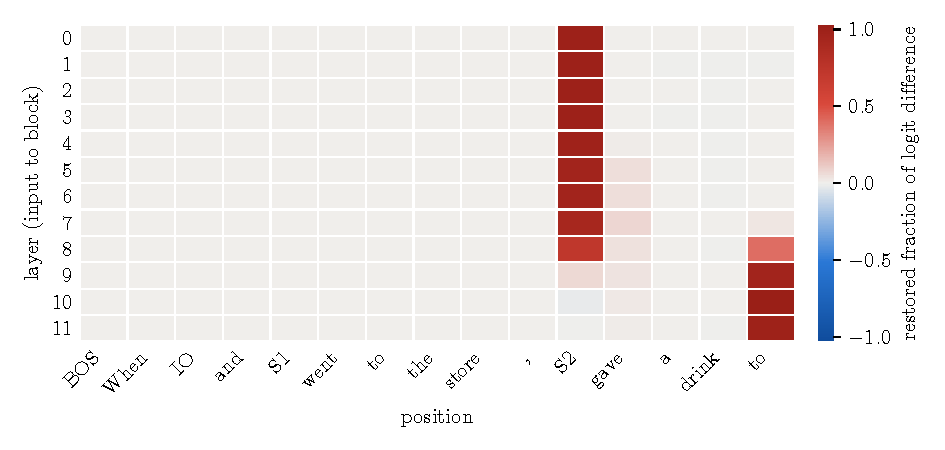
\includegraphics[width=0.86\textwidth]{figures/fig_resid_patching.pdf}
\caption{Activation patching of the residual stream of GPT-2 small on the IOI task. Each cell shows the
denoising effect \eqref{eq:denoise} of the stream at the input of one layer at one position, averaged over 12
pairs of prompts. IO is the indirect object, S1 and S2 are the two occurrences of the subject.}
\label{fig:residpatch}
\end{figure}

\begin{caution}
The corrupted prompt decides what a patching experiment can find. Ours changes which name is repeated and keeps
everything else. Components that are needed for the task and behave the same on both prompts, for example
whatever establishes that the next token should be a name at all, stay invisible. A different question requires
a different pair of prompts. \citet{zhang2024towards} and \citet{heimersheim2024use} discuss these choices in
detail.
\end{caution}

\subsection{Sufficient, necessary, direct, total}
\label{sec:necessity}

We now take the output of each attention head, at all positions, as a node. \Cref{tab:heads} lists four numbers
for twelve heads from the classes of \citet{wang2023interpretability}. The classes are explained in
\cref{sec:ioi}, and for the moment they are only labels. The first is the direct logit attribution from \cref{sec:lens}. The second
is the denoising effect \eqref{eq:denoise}. The last two describe the noising experiment in logits. The
\emph{total effect} is the numerator of \eqref{eq:noise}, which is the drop of the metric when the head receives
its corrupted output. The \emph{direct effect} is the part of this drop that comes from the head's own summand
in \eqref{eq:dla-ld}, computed with the final scale held fixed. A negative entry in the table belongs to a head
that works against the correct name: restoring it lowers the metric, and corrupting it raises the metric. The
effects of different heads do not add up to one, because the heads depend on each other. For head 9.9 the direct
effect of $7.00$ is about twice its DLA, because in the corrupted run this head writes with similar strength in
favour of the other name.

\begin{table}[t]
\centering\small
\begin{tabular}{@{}llrrrr@{}}
\toprule
 & & & denoising & \multicolumn{2}{c}{noising (logits)} \\
\cmidrule(l){5-6}
Head & Class in \citet{wang2023interpretability} & DLA & effect & direct effect & total effect \\
\midrule
9.9 & name mover & $3.57$ & $0.29$ & $7.00$ & $1.40$ \\
9.6 & name mover & $1.10$ & $0.01$ & $2.27$ & $-0.77$ \\
10.0 & name mover & $0.59$ & $0.09$ & $1.31$ & $0.57$ \\
10.7 & negative name mover & $-2.52$ & $-0.52$ & $-4.62$ & $-3.83$ \\
11.10 & negative name mover & $-1.05$ & $-0.28$ & $-2.24$ & $-2.15$ \\
\addlinespace
8.6 & S-inhibition & $0.00$ & $0.37$ & $0.01$ & $1.55$ \\
8.10 & S-inhibition & $0.44$ & $0.34$ & $0.73$ & $1.51$ \\
7.9 & S-inhibition & $0.19$ & $0.22$ & $0.42$ & $1.17$ \\
7.3 & S-inhibition & $0.22$ & $0.14$ & $0.42$ & $0.96$ \\
\addlinespace
5.5 & induction & $0.00$ & $0.33$ & $0.00$ & $1.46$ \\
6.9 & induction & $0.00$ & $0.15$ & $0.00$ & $0.37$ \\
3.0 & duplicate token & $0.00$ & $0.15$ & $0.00$ & $0.45$ \\
\bottomrule
\end{tabular}
\caption{Four views of twelve attention heads of GPT-2 small on the IOI task, averaged over 12 pairs of prompts.
DLA is in logits, the denoising effect is a fraction of the gap of $8.04$ logits between the clean and the
corrupted run, and the two noising columns are in logits. The classes are those assigned by
\citet{wang2023interpretability}.}
\label{tab:heads}
\end{table}

The table contains three lessons that hold far beyond this example.

\paragraph{Lesson 1: direct attribution misses the early part of a mechanism.} Heads 8.6, 5.5, 6.9 and 3.0 have a
DLA of zero. They write nothing in the direction that separates the two names at the output. Yet corrupting head 8.6 or head 5.5 alone costs
about $1.5$ logits. These heads matter through what later heads do with their output. Only an intervention
reveals them.

\paragraph{Lesson 2: the total effect can be much smaller than the direct effect.} Corrupting the name mover 9.9
removes $7.00$ logits of direct contribution, and the metric drops by only $1.40$. Four fifths of the damage is
undone by the layers after it. For head 9.6 the total effect is even negative: the model does slightly better
when this helpful head is corrupted. \citet{wang2023interpretability} observed the same phenomenon and found
heads that take over when the name movers are removed, which they call backup name movers.
\citet{mcgrath2023hydra} studied such compensation systematically under the name \emph{hydra effect}. The
consequence is uncomfortable: removing a component and seeing little change does not show that the component
is unimportant.

\paragraph{Lesson 3: noising and denoising answer different questions.} Denoising asks whether the clean value
of one node is \emph{sufficient} to move a corrupted run towards the clean behaviour. Noising asks whether the
clean value of one node is \emph{necessary} for the clean behaviour. If several components do the same job in
parallel, each is sufficient and none is necessary. If several components are needed jointly, each is necessary
and none is sufficient. \Cref{ex:andor} makes this exact in a model with two nodes.

\paragraph{Paths.} Patching a node changes everything downstream of it. To learn through \emph{which} later
components a node acts, we patch along selected paths only. For example, to measure the effect of head 8.6
that passes through head 9.9, we recompute the input of head 9.9 with the corrupted output of head 8.6 and
keep the clean value on every other path. This is \emph{path patching}
\citep{wang2023interpretability,goldowskydill2023localizing}. The direct effect in \cref{tab:heads} is the
special case of the path that leads straight to the output.

\begin{remark}[A clash of terminology]
In causal mediation analysis \citep{pearl2001direct,vig2020investigating} the treatment is the change of the
\emph{input}, and the ``indirect effect'' through a mediating node is the part of the change of the output that
passes through that node. This is what activation patching measures. It should not be confused with our use of
``direct'', which refers to the path from a \emph{component} to the output that avoids all later components.
\end{remark}

\subsection{Attribution patching: a linear shortcut}
\label{sec:attrpatching}

Patching costs one run of the model per node. For 144 heads this is nothing. For every neuron at every position,
or for millions of SAE latents, it is prohibitive. \emph{Attribution patching}
\citep{nanda2023attribution,syed2024attribution} estimates all patching effects at once.

Fix a node $g$ and regard the metric of the corrupted run as a function of the value written to $g$. A
first-order Taylor expansion of this function around the value $g(\corr)$ gives
\begin{equation}\label{eq:attrpatch}
M\big(\corr \mid g\leftarrow g(\clean)\big)-M(\corr) \;\approx\;
\big(g(\clean)-g(\corr)\big)^\top\,\nabla_gM(\corr),
\end{equation}
where $\nabla_gM(\corr)$ is the gradient of the metric with respect to the node, evaluated in the unmodified
corrupted run. The right-hand side needs the values of all nodes on both prompts, which two forward passes
provide, and the gradients with respect to all nodes, which a single backward pass provides. The cost no longer
depends on the number of nodes.

\Cref{fig:attrpatch} compares the estimate with the exact denoising effect for all 144 heads of the running
example. The correlation is $0.98$. The estimate identifies the same heads. Its largest errors occur for two
heads with large effects. For head 9.9 it gives $0.43$ where the exact value is $0.29$, and for head 5.5 it gives
$0.25$ where the exact value is $0.33$.

\begin{figure}[t]
\centering
\begin{minipage}[c]{0.44\textwidth}
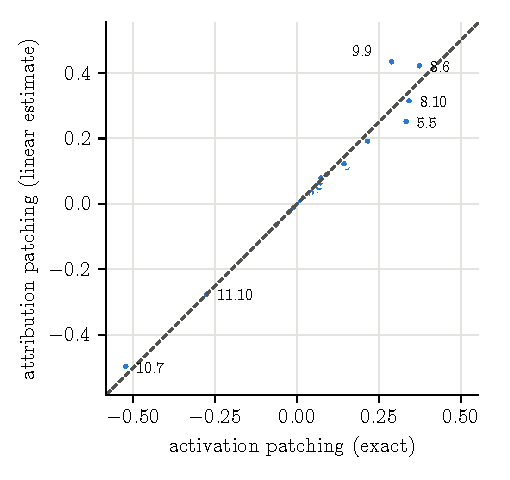
\includegraphics[width=\textwidth]{figures/fig_attr_vs_act.pdf}
\end{minipage}\hfill
\begin{minipage}[c]{0.5\textwidth}
\caption{Attribution patching against activation patching for the 144 attention heads of GPT-2 small on the IOI
task. Each dot is one head. The horizontal axis is the exact denoising effect \eqref{eq:denoise}, and the
vertical axis is the linear estimate \eqref{eq:attrpatch} divided by the same gap. Dots on the dashed diagonal
are estimated without error.}
\label{fig:attrpatch}
\end{minipage}
\end{figure}

\begin{caution}
The estimate \eqref{eq:attrpatch} is a linearisation, and it fails where the model is far from linear between
the two values. The standard example is a saturated attention pattern. If a head puts almost all its weight on
one source, the gradient with respect to the scores is almost zero, although a large change of the scores
would redirect the head completely. \citet{kramar2024atp} analyse such cases and propose corrections. In
practice the estimate serves as a fast filter, and the nodes that it selects are then patched exactly.
\end{caution}

\subsection{Steering}
\label{sec:steering}

Patching replaces an activation by one that occurred on another prompt. \emph{Steering} moves an activation
along a chosen direction and tests in this way whether the direction controls a behaviour. Let $v\in\R^d$ be a
unit vector. There are two basic operations on a stream vector $x$.
\begin{align}
\text{activation addition:}\qquad & x \;\longmapsto\; x+\eta\,v,\qquad \eta\in\R, \label{eq:actadd}\\
\text{directional ablation:}\qquad & x \;\longmapsto\; x-(v^\top x)\,v . \label{eq:dirabl}
\end{align}
The first adds the direction with a strength $\eta$ \citep{turner2023steering,rimsky2024steering,zou2023representation}.
The second removes the component of $x$ along $v$: the result has inner product
$v^\top x-(v^\top x)\,v^\top v=0$ with $v$. The direction can come from any of the earlier sections: a difference of
means \eqref{eq:diffmeans}, a probe, or a dictionary direction of an SAE.

A clear case is the study of refusal by \citet{arditi2024refusal}. Chat models are trained to refuse harmful
requests. The authors collected stream activations on harmful and on harmless instructions and took the
difference of the two means at one layer as the direction $v$. In 13 open chat models with up to 72 billion
parameters, they obtained the same two results. With \eqref{eq:dirabl} applied at all layers and positions, the
model no longer refused harmful requests. With \eqref{eq:actadd} applied at the layer where $v$ was extracted,
the model refused harmless ones. In these models the decision to refuse passes through one direction.

Results of this kind are the strongest evidence for the linear representation hypothesis of \cref{sec:lrh},
because they are causal: a direction found by observation changes the behaviour in the predicted way when it is
manipulated. They are also the basis of practical applications, since a direction that controls a behaviour
can be used to monitor or to adjust it.

\begin{caution}
Steering has its own failure modes. A large $\eta$ produces activations that the model never sees in normal
operation, and its text degrades. A direction estimated from data contains whatever else differs between the
two classes of prompts, as \eqref{eq:diffmeans} shows, so the behaviour may change for another reason than the
intended one. An evaluation should therefore measure three things: whether the intended behaviour changes,
whether unrelated behaviour stays intact, and how the method compares with simple baselines such as changing
the prompt \citep{wu2025axbench}.
\end{caution}

\subsection{Testing a hypothesis about an algorithm}
\label{sec:abstraction}

Patching single nodes localises a behaviour. A full explanation claims more: that the model implements a
particular algorithm, with named intermediate variables that are stored at particular places. \emph{Causal
abstraction} \citep{geiger2021causal,geiger2025causal} turns such a claim into an experiment. Suppose the
hypothesis says that a certain set of activations stores the variable ``the name that is repeated''. We take two
prompts with different repeated names and patch exactly these activations from the second run into the first.
The hypothesis predicts the new output: it must be what the algorithm returns when this one variable is swapped
and all others are kept. The fraction of prompt pairs on which the model agrees with the prediction is called
the interchange intervention accuracy. Causal scrubbing \citep{chan2022causal} is a related test based on
resampling.

The variable need not be stored in individual neurons or heads. Distributed alignment search
\citep{geiger2024finding} looks for it in a subspace of the stream, and finds the subspace by gradient descent on
the interchange accuracy. This added power has a price. \citet{makelov2024subspace} show that a subspace found
by optimisation can produce the predicted behaviour by activating a pathway that the model does not normally
use. The intervention then succeeds, and the explanation is still wrong. The more freedom a method has in
choosing where and how to intervene, the more carefully its result has to be checked against how the model
behaves without the intervention.

\begin{takeaways}
An intervention overwrites a node and recomputes the rest. The replacement value defines the question.
Activation patching uses the value from a minimally different prompt and localises the information that
distinguishes the two prompts. Direct effects, total effects, sufficiency and necessity are four different
quantities, and compensation by later layers can hide important components. Attribution patching approximates
all patching effects with two forward passes and one backward pass. Steering tests whether a direction controls
a behaviour.
\end{takeaways}

\begin{exercise}\label{ex:andor}
A model has two binary nodes $g_1,g_2$. On the clean prompt both are $1$, on the corrupted prompt both are $0$.
Compute the denoising effect \eqref{eq:denoise} and the noising effect \eqref{eq:noise} of $g_1$ when the metric
is (a) $M=\max(g_1,g_2)$ and (b) $M=\min(g_1,g_2)$. Relate the result to Lesson 3.
\end{exercise}
\begin{exercise}\label{ex:affine}
Show that \eqref{eq:attrpatch} holds with equality if the metric of the intervened run is an affine function of
the value written to $g$. Give an example of a node and a metric in a transformer for which this is the case.
\end{exercise}
\begin{exercise}\label{ex:projection}
Show that directional ablation \eqref{eq:dirabl} with a unit vector $v$ is linear in $x$, that applying it twice
is the same as applying it once, and that it does not change the read-out $w^\top x$ of a probe direction $w$
that is orthogonal to $v$.
\end{exercise}
